\documentclass[10pt,landscape]{article}
\usepackage{multicol}
\usepackage{calc}
\usepackage{ifthen}
\usepackage[landscape]{geometry}
\usepackage{listings}
\usepackage{amsmath,amsthm,amsfonts,amssymb}
\usepackage{mathtools}
\usepackage{color,graphicx,overpic}
\usepackage{hyperref}
\usepackage[dvipsnames]{xcolor}

\usepackage{MnSymbol}
\usepackage{graphicx}
\usepackage{wrapfig}
\usepackage{tikz}

\usepackage{blindtext}

% This sets page margins to .1 inch if using letter paper, and to 1cm
% if using A4 paper. (This probably isn't strictly necessary.)
% If using another size paper, use default 1cm margins.
\ifthenelse{\lengthtest { \paperwidth = 11in}}
    { \geometry{top=0.2in,left=0.2in,right=0.2in,bottom=0.2in} }
    {\ifthenelse{ \lengthtest{ \paperwidth = 297mm}}
        {\geometry{top=1cm,left=1cm,right=1cm,bottom=1cm} }
        {\geometry{top=1cm,left=1cm,right=1cm,bottom=1cm} }
    }

% Turn off header and footer
\pagestyle{empty}

% Redefine section commands to use less space
\makeatletter
\renewcommand{\section}{\@startsection{section}{1}{0mm}%
                                {-1ex plus -.5ex minus -.2ex}%
                                {0.5ex plus .2ex}%x
                                {\normalfont\large\bfseries}}
\renewcommand{\subsection}{\@startsection{subsection}{2}{0mm}%
                                {-1ex plus -.5ex minus -.2ex}%
                                {0.5ex plus .2ex}%
                                {\normalfont\normalsize\bfseries}}
\renewcommand{\subsubsection}{\@startsection{subsubsection}{3}{0mm}%
                                {-1ex plus -.5ex minus -.2ex}%
                                {0.5ex plus .2ex}%
                                {\normalfont\footnotesize\bfseries}}
\makeatother

% Itemize to use less space
\usepackage{enumitem}
\setlist{leftmargin=*, nosep}
\setenumerate{nosep}

% Define BibTeX command
\def\BibTeX{{\rm B\kern-.05em{\sc i\kern-.025em b}\kern-.08em
    T\kern-.1667em\lower.7ex\hbox{E}\kern-.125emX}}

% Don't print section numbers
\setcounter{secnumdepth}{0}


\setlength{\parindent}{0pt}
\setlength{\parskip}{0pt plus 0.5ex}

%My Environments
\newtheorem{example}[section]{Example}

\newcommand{\Blue}[1]{\noindent{\textcolor{Blue}{\textbf{#1}}}:}
\newcommand{\Red}[1]{\noindent{\textcolor{BrickRed}{\textbf{#1}}}:}
\newcommand{\Green}[1]{\noindent{\textcolor{PineGreen}{\textbf{#1}}}:}
\newcommand{\Hint}[1]{\noindent{\textcolor{Orange}{#1}}}
% -----------------------------------------------------------------------

\begin{document}
\raggedright
\scriptsize

\begin{multicols}{4}
% multicol parameters
% These lengths are set only within the two main columns
%\setlength{\columnseprule}{0.25pt}
\setlength{\premulticols}{1pt}
\setlength{\postmulticols}{1pt}
\setlength{\multicolsep}{1pt}
\setlength{\columnsep}{2pt}

\subsubsection{Consumer Demand}

\Blue{Willingness To Pay (WTP)} The most a consumer will pay for a good.

\Red{Consumer Demand} For each price $P$ what quantity is demanded? $Q = Q_D (P)$. \textbf{Inverse demand}: the price at which quantity Q could be sold. $P = P_D (Q)$
\Hint{\textbf{Remember!} Given $Q(P)$, \underline{inverse} it to plot $P(Q)$!}

\Red{Consumer Surplus} Area below demand curve and above price paid.

\Blue{Elasticity} meansure of price sensitivity
\Green{Own-price elasticity of demand $\frac{\% \Delta Q_1^D}{\% \Delta P_1}$} the \% change in quantity demanded for a
1\% change in its price. Always negative by Law of Demand. $|E| \begin{cases}
    < 1 & \text{Inelastic} \\
    > 1 & \text{Elastic}
\end{cases}$

\Green{Cross-price elasticity of demand $\frac{\% \Delta Q_1^D}{\% \Delta P_2}$} the \% change in quantity demanded for a
1\% change in \underline{another good's} price. $\begin{cases}
    > 0 & \text{SUBSTITUTES (wine \& beer)} \\
    < 0 & \text{COMPLEMENTS (popcorn \& beer)}
\end{cases}$

\subsubsection{Demand Estimation}

\Red{Demand Shifts} Any change in the envrionment that changes demand other than price. E.g. before and after advertising.

\Blue{Estimation Techniques}
\begin{enumerate}
    \item Randomized Control Trials: A/B tests. Considered the \underline{gold standard} for demand estimation because
        of their ability to establish causality. In a randomized experiment, subjects are randomly allocated to
        different prices and this allows us to attribute the change in demand to price changes rather than to some other
        confounding variable.
    \item ``Nautral'' or ``Quasi-'' experiments: when price variation is ``as good as random'' (e.g. demand just above
        or below price-surge threshold).
\end{enumerate}

\Green{Equity Tradeoffs} different equity objectives may exist in different applications. Continuous algorithmic
testing, penalties for disparities, affirmative information potential solutions.

\subsubsection{Costs}

\Blue{Sunk Cost} costs that are unavoidable and cannot be recovered. Whether a cost is sunk or not depends on the timing
of the business decision.

\Blue{Opportunity Cost} the highest valued alternative use of an input; an example is ``no such thing as a free lunch'':
you could do something else with your time. Example of Capital: Rate of return on the next best alternative use of funds
(relative to the current business decision).

\Blue{Fixed Cost} costs that don't vary with the level of output (Q).

\Blue{Variable Cost} costs that vary with the level of output (Q).

The fixed vs variable cost distinction depends on the business question and on the time horizon. E.g., all inputs
(including capacity) are variable in the ``Long Run''

\Red{Economies of Scale} average cost ($\frac{\text{TC}}{Q}$) falls with higher Q.
Why a firm might have EoS:
\begin{itemize}
    \item fixed cost is spread out over more units
    \item different technology / specialization is used at larger scale
    \item greater bargaining power lowering input prices
    \item Learning curve could be sped up as well (although this would shift the AC curve) whereas EoS is about moving
        along an AC curve.
\end{itemize}

\Green{Net Present Value (NPV)} multiply all future cash flows by $\frac{1}{(1+r)^t}$ and add them up, where $r =$
annual interest rate (opportunity cost of capital) and $t =$ number of years in the future. E.g.:
\begin{itemize}
    \item If the opportunity cost of capital is 10\% per annum, a startup cost of 280 and annual flow expenditures of
        100 for 3 years (beginning next year):
        $NPV = -\frac{280}{1.1} - \frac{100}{1.1} - \frac{100}{1.21} - \frac{100}{1.331} = -503$
    \item If the opportunity cost of capital is 10\% per annum, an annual flow expenditures of 200 for 3 years
        (beginning next year):
        $NPV = - \frac{200}{1.1} - \frac{200}{1.21} - \frac{200}{1.331} = -497$
\end{itemize}

\subsubsection{Sources of Market Power}

\Red{Barriers to entry} e.g. large fixed costs

\Red{Network Externality} The product is more valuable to you if it is used by others. To maintain n.e., (1) establish
switching costs (2) interoperability (weakens direct n.e.)
\begin{itemize}
    \item Direct n.e.: Emails -- requires other users
    \item Indirect n.e.: Windows -- requires complements like software developed for Win.
\end{itemize}
\Blue{Positive N.E.} the value of a product increases with the \# of users (higher WTP). Network goods. Makes demand \textit{more
elastic} so an aggressive pricing strategy becomes more profitable.
\Blue{Negative N.E.} e.g. luxury goods.

\Red{Learning Curve} Average costs falls with experience. Commonly discussed as: AC falls $X\%$ with a doubling of
output (e.g., manufacturing processes have strong learning effects.) Google Search has strong learning effects: more
experience $\rightarrow$ more data $\rightarrow$ better machine learning for search algorithm and targeted advertising.

\subsubsection{Monopoly Pricing}

\Red{Monopoly} a single firm is in the market.

\Blue{Marginal Cost (MC)} How cost changes as output $Q$ changes: for 1 unit, $Cost(Q) - Cost(Q-1)$ ; for more units,
$\frac{\Delta Cost}{\Delta Q}$; and for small changes, $\frac{d Cost}{d Q}$. \Hint{Fixed costs don't enter MC.}

\Blue{Marginal Revenue (MR)} in order to sell more units, the price must be lowered for all units.
\begin{wrapfigure}{r}{0.4\columnwidth}
    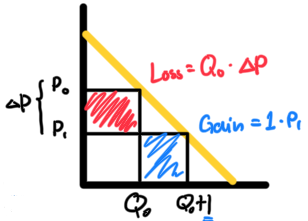
\includegraphics[width=0.4\columnwidth]{MR.png}
\end{wrapfigure}
\fbox{$MR = \frac{\Delta Rev(Q)}{\Delta Q} = P(Q) + Q \frac{\Delta P(Q)}{\Delta Q}$}
Decrease price results in: \textbf{\textcolor{Blue}{gain}} in Rev from Q increases + \textbf{\textcolor{Red}{loss}} in Revenue from P reduction for all units.
\Hint{If demand curve linear, MR has same intercept and twice the slope. $P(Q) = 100 - Q \rightarrow MR = 100 - 2 Q$}

\begin{multicols}{2}
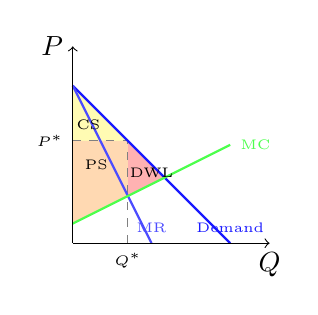
\begin{tikzpicture}
    % CS
    \fill[yellow!30] (0, 1.3) -- (0.7, 1.3) -- (0, 2) -- cycle;

    %DWL
    \fill[red!30] (0.7, 0.6) -- (0.7, 1.3) -- (1.167, 0.833) -- cycle;

    %PS
    \fill[orange!30] (0, 0.25) -- (0, 1.3) -- (0.7, 1.3) -- (0.7, 0.6) -- cycle;

    \draw[dashed,gray] (0, 1.3) -- (0.7, 1.3);
    \draw[dashed,gray] (0.7, 0) -- (0.7, 1.3);
    \draw[thick,blue!90] (0,2) -- (2,0) node[anchor=south] {\tiny Demand}; % D
    \draw[thick, blue!70] (0,2) -- (1,0) node[anchor=south] {\tiny MR}; % MR
    \draw[thick, green!70] (0,0.25) -- (2,1.25) node[anchor=west] {\tiny MC}; % MC
    % Draw axes
    \draw[->] (0,0) -- (2.5,0) node[anchor=north] {$Q$};
    \draw[->] (0,0) -- (0,2.5) node[anchor=east] {$P$};
    
    % Label values
    \node[anchor=north] at (0.7,0) {\tiny $Q^*$};
    \node[anchor=east] at (0,1.3) {\tiny $P^*$};
    \node at (0.2,1.5) {\tiny CS};
    \node at (0.3,1) {\tiny PS};
    \node at (1,0.9) {\tiny DWL};

\end{tikzpicture}

\Green{Profix Maximization} optimal $Q^*$ when $MC(Q^*) = MR(Q^*)$. Then solve for optimal price $P^* =P(Q^*)$
\Hint{Does not depend on the level of demand.}

\Green{Mark-up Formula} resulting from profit-max, $P^*$ satisfies: $\frac{P-MC}{P} = -\frac{1}{\epsilon}$ ($\epsilon$ is the demand elasticity).
\Hint{Relatively more elastic markets (markets with more price-sensitive consumers) will face smaller markups} (i.e., lower prices if costs are the same across markets).
\end{multicols}

\subsubsection{Consumer Self-Selection and Two-Part Tariffs}

\Red{Price Discrimination} requires \begin{itemize}
    \item Market power (competition undermines price discrimination)
    \item Knowledge about the customer: seller needs \textit{data}
    \item No re-sale (to prevent arbitrage)
\end{itemize}

\begin{wrapfigure}{r}{0.4\columnwidth}
    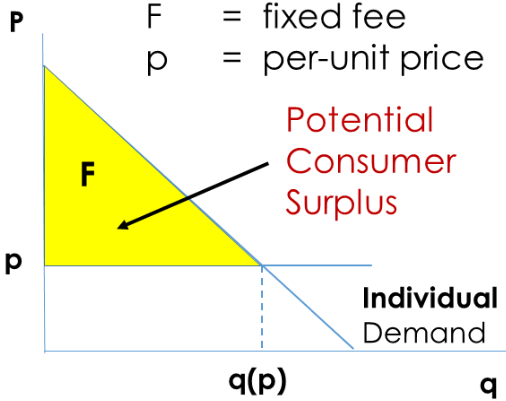
\includegraphics[width=0.4\columnwidth]{TwoPartTariff.png}
\end{wrapfigure}
\Red{Two-Part Tarriff} Charge 2 prices: access fee ($F$) and per-unit price ($p$)
\Hint{A consumer pays a two-part tariff if their Total WTP at that price $\ge F + P \cdot Q$}, where $Q$ is the quantity
they would consume at price $P$ (can get $Q$ from their demand curve).

\Green{Two-Part Tariff with One Type of Customer} If $MC=0$, optimal: $p^* = 0$ and $F^* = \text{total WTP}$.
If $MC > 0$, optimal: $p^* = MC$ and $F^* = \text{\textcolor{Yellow}{CS} when p=MC}$.

\Green{Two-Part Tariff with Multiple Types of Customers} $F$ affects all buyers the same, but $p$ extracts more out of
high WTP buyers since they buy more. Set $F$ to the lowest $CS$ of all types.

\begin{multicols}{2}
e.g., Amusement park: $Q_t = 20 - P$, $Q_r = 10 - \frac{P}{2}$ ($Q$: \# of rides demanded). Issue ``Value'' (10 rides
max) intended for $r$ and ``Unlimited'' intended for $t$, both with zero price per ride. Then
$F_{\text{Value}} = CS_r = 0.5 \cdot 20 \cdot 10 = 100$
$F_{\text{Unlimited}} = \textcolor{red!50}{CS_r} + \textcolor{blue!50}{\text{Upgrade Price}} = 100 + 50 = 150$

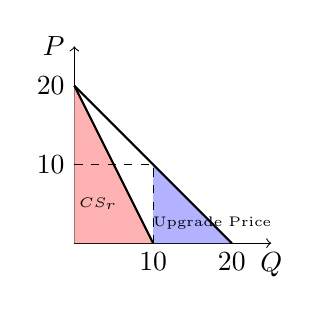
\begin{tikzpicture}

    % Draw axes
    \draw[->] (0,0) -- (2.5,0) node[anchor=north] {$Q$};
    \draw[->] (0,0) -- (0,2.5) node[anchor=east] {$P$};

    \fill[red!30] (0,0) -- (0,2) -- (1,0) -- cycle; % CS_r
    \fill[blue!30] (1,0) -- (1,1) -- (2,0) -- cycle; % Upgrade
    
    \draw[thick] (2,0) -- (0,2);
    \draw[thick] (1,0) -- (0,2);
    \draw[dashed] (1,0) -- (1,1);
    \draw[dashed] (0,1) -- (1,1);

    \node[anchor=north] at (2,0) {$20$};
    \node[anchor=north] at (1,0) {$10$};
    \node[anchor=east] at (0,2) {$20$};
    \node[anchor=east] at (0,1) {$10$};

    % Label the regions
    \node at (0.3,0.5) {\tiny $CS_r$};
    \node at (1.75,0.25) {\tiny Upgrade Price};

\end{tikzpicture}
\end{multicols}

\subsubsection{Product Portfolios}
Consumers maximize surplus so they pick a choice with higher CS out of multiple (products/two-part tarrifs).
\Hint{By reducing the quality of its low-end goods, a firm can often make these goods much less attractive for high WTP
buyers, while having a comparatively smaller effect on the value to low WTP buyers.} For any given portfolio of products:
\begin{enumerate}
    \item For \textbf{each consumer type} (e.g. H and L) and for \textbf{for each choice} (e.g. S and I), compute CS and
        they will buy the choice with highest CS.
    \item Estimate profits from \textbf{each consumer type} from buying their preferred choice. Multiply profit per
        consumer from that type with the \# of such type to get total profit from this consumer type.
    \item Add up profits across all consumer types.
    \item \textbf{Check}: are consumers buying the product you are targeting with? \begin{itemize}
        \item No: adjust product portfolio and/or price; then re-estimate above.
        \item Yes: try adjusting prices such that the \textbf{Check} still holds \textit{AND} profits increase.
    \end{itemize}
\end{enumerate}
\begin{tabular}{|c|c|c|}
    \hline
    Consumer WTP & \textbf{S}uperior Prod & \textbf{I}nferior Prod \\ \hline
    Type H & 5000 & 2000 \\
    Type L & 3000 & 1000 \\ \hline
\end{tabular}
To max value extraction serving \underline{both markets}:
\begin{enumerate}
    \item Set $P_{I} = WTP_{L,I} = \$1000$
    \item Set $P_{S} = WTP_{H,S} - CS_{H,I}= \$5000 - (\$2000 - \$1000) = \$4000$
\end{enumerate}

\subsubsection{Strategic Pricing \& Bundling}

\Red{Bundling} practice of selling different goods in a package.

\Blue{Bundled discount} a price reduction (relative to single-product prices) for a customer who buys a specified
combination of products.

\Hint{In graphes: each point's coordinates are one consumer's WTP on A and B. $\overline{V_A}$ and $\overline{V_B}$: highest WTPs any customers have for A and B.}
\begin{multicols}{2}
\Blue{Individual pricing} separate decisions for each product.

\begin{itemize}
    \item buy A if $V_A \ge p_A$
    \item buy B if $V_B \ge p_B$
\end{itemize}

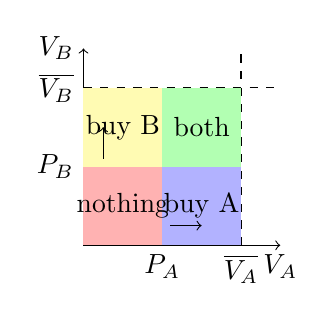
\begin{tikzpicture}

    % Draw axes
    \draw[->] (0,0) -- (2.5,0) node[anchor=north] {$V_A$};
    \draw[->] (0,0) -- (0,2.5) node[anchor=east] {$V_B$};

    % Dashed lines for the boundaries
    \draw[dashed] (2,0) -- (2,2.5);
    \draw[dashed] (0,2) -- (2.5,2);

    % Labels for P_A and P_B
    \node[anchor=north] at (1,0) {$P_A$};
    \node[anchor=east] at (0,1) {$P_B$};

    % Draw the regions
    \fill[red!30] (0,0) rectangle (1,1); % buy nothing
    \fill[blue!30] (1,0) rectangle (2,1); % buy A
    \fill[yellow!30] (0,1) rectangle (1,2); % buy B
    \fill[green!30] (1,1) rectangle (2,2); % buy both

    % Label the regions
    \node at (0.5,0.5) {nothing};
    \node at (1.5,0.5) {buy A};
    \node at (0.5,1.5) {buy B};
    \node at (1.5,1.5) {both};

    % Arrows for directions
    \draw[->] (1.1, 0.25) -- (1.5, 0.25);
    \draw[->] (0.25, 1.1) -- (0.25, 1.5);

    % Labels for \overline{V_A} and \overline{V_B}
    \node[anchor=north] at (2,0) {$\overline{V_A}$};
    \node[anchor=east] at (0,2) {$\overline{V_B}$};
\end{tikzpicture}
\end{multicols}

\begin{multicols}{2}
\Blue{Pure bundling} only the total value of the bundle matters. Buy bundle if $V_A + V_B \ge P_\text{bundle}$
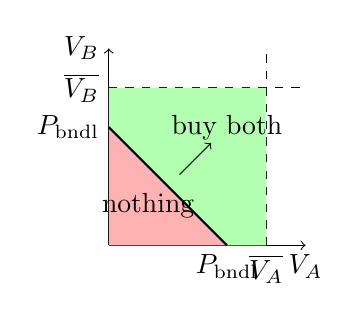
\begin{tikzpicture}
    % Draw axes
    \draw[->] (0,0) -- (2.5,0) node[anchor=north] {$V_A$};
    \draw[->] (0,0) -- (0,2.5) node[anchor=east] {$V_B$};

    % Dashed lines for the boundaries
    \draw[dashed] (2,0) -- (2,2.5);
    \draw[dashed] (0,2) -- (2.5,2);

    % Labels for P_bundle
    \node[anchor=north] at (1.5,0) {$P_{\text{bndl}}$};
    \node[anchor=east] at (0,1.5) {$P_{\text{bndl}}$};

    % Draw the regions
    \fill[red!30] (0,0) -- (0,1.5) -- (1.5,0) -- cycle; % buy nothing
    \fill[green!30] (0,1.5) -- (0,2) -- (2,2) -- (2,0) -- (1.5,0) -- cycle; % buy both

    % Draw the diagonal boundary (halved coordinates)
    \draw[thick] (0,1.5) -- (1.5,0);

    % Label the regions
    \node at (0.5,0.5) {nothing};
    \node at (1.5,1.5) {buy both};

    % Arrow for directional indication
    \draw[->] (0.9,0.9) -- (1.3,1.3);

    % Labels for \overline{V_A} and \overline{V_B}
    \node[anchor=north] at (2,0) {$\overline{V_A}$};
    \node[anchor=east] at (0,2) {$\overline{V_B}$};
\end{tikzpicture}
\end{multicols}

\begin{multicols}{2}
\Blue{Mixed bundling} choose the option that gives you the highest CS. $P_{\text{bndl}} = P_A + P_B - D$.
Choose max out of:
\begin{itemize}
    \item $0$ nothing
    \item $V_A-P_A$ A only
    \item $V_B-P_B$ B only
    \item $V_A + V_B - P_{\text{bndl}}$ bundle
\end{itemize}
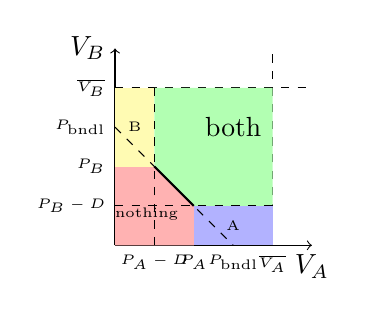
\begin{tikzpicture}
    % Draw axes
    \draw[->] (0,0) -- (2.5,0) node[anchor=north] {$V_A$};
    \draw[->] (0,0) -- (0,2.5) node[anchor=east] {$V_B$};

    % Dashed lines for the boundaries
    \draw[dashed] (2,0) -- (2,2.5);
    \draw[dashed] (0,2) -- (2.5,2);

    % Labels for P_bundle, P_A, P_B, P_A-D, and P_B-D
    \node[anchor=north] at (1,0) {\tiny $P_A$};
    \node[anchor=north] at (0.5,0) {\tiny $P_{A} - D$};
    \node[anchor=north] at (1.5,0) {\tiny $P_{\text{bndl}}$};

    \node[anchor=east] at (0,1) {\tiny $P_B$};
    \node[anchor=east] at (0,0.5) {\tiny $P_{B} - D$};
    \node[anchor=east] at (0,1.5) {\tiny $P_{\text{bndl}}$};

    % Draw the regions
    \fill[red!30] (0,0) -- (0,1) -- (0.5,1) -- (1,0.5) -- (1,0) -- cycle; % buy nothing
    \fill[blue!30] (1,0) -- (2,0) -- (2,0.5) -- (1,0.5) -- cycle; % buy only A
    \fill[yellow!30] (0,1) -- (0,2) -- (0.5,2) -- (0.5,1) -- cycle; % buy only B
    \fill[green!30] (1,0.5) -- (2,0.5) -- (2,2) -- (0.5, 2) -- (0.5, 1) -- cycle; % buy both

    % Draw the thick line dividing "buy nothing" and "buy only A"
    \draw[dashed] (0,1.5) -- (1.5,0);
    \draw[dashed] (0,0.5) -- (2, 0.5);
    \draw[dashed] (0.5,0) -- (0.5,2);
    \draw[thick] (1,0.5) -- (0.5,1);

    % Label the regions
    \node at (0.4,0.4) {\tiny nothing};
    \node at (0.25,1.5) {\tiny B};
    \node at (1.5,1.5) {both};
    \node at (1.5,0.25) {\tiny A};

    % Labels for \overline{V_A} and \overline{V_B}
    \node[anchor=north] at (2,0) {\tiny $\overline{V_A}$};
    \node[anchor=east] at (0,2) {\tiny $\overline{V_B}$};
\end{tikzpicture}
\end{multicols}

\subsubsection{Adverse Selection}

Arises when the buyers who are costlier to serve are also the ones who are most inclined to purchase, and firms \textbf{cannot
tell which consumers are higher} vs. lower cost to serve. Affects markets across sectors and product type e.g.
insurance, cars, restaurants, as long as lack of information on “good” vs. “bad” risks. In extreme cases, adverse
selection can make it impossible for a firm to sell a product profitably.
If higher WTP customers are also higher cost to serve while we need to price above the AC, it's
\textcolor{red}{impossible} to find such price.

\Blue{Firm-level solutions} (i) Add information (screening \& signaling) about which consumers are high vs. low cost to
serve; (ii) Warrenties, reputation, advertising; (iii) Strategic pricing: Premium, deductible and co-pay.

\Blue{Policy-level solutions} (i) Lemons Laws; (ii) BBB (firm reputation); (iii) Risk Pooling e.g. health insurance
prices set at the community level, insurance mandates.

\end{multicols}
\end{document}